
\begin{refsection}
\startcontents[chapters]	
\chapter{Game theory \& multiobjective optimization}\label{ch:game-theory}	
\printcontents[chapters]{}{1}{}
\section{Static games with complete information}
\subsection{Normal form game concepts}
\begin{definition}[normal-form game]\index{normal-form game}  
\cite[3]{leyton2008essentials}A (finite, n-person) normal-form game is a tuple $(N,A,u)$, where
\begin{itemize}
    \item N is the number of players, indexed by $i=1,2,...,N$;
    \item $A=A_1\times A_2 ...\times A_N$, where $A_i$ is the action/strategy space for player i. An element $a = (a_1,a_2,...,a_N) \in A$ is called the action profile;
    \item $u=(u_1,u_2,...,u_n)$ where $u_i = u_i(a_1,a_2,...,a_N)$ is the \textbf{utility/payoff function} for player $i$. 
\end{itemize}
\end{definition}

\begin{definition}[common-payoff games, coordinated games]
\cite[4]{leyton2008essentials}A common-payoff game is a normal-form game in which for \textbf{all} action profiles $a\in A$ and \textbf{any} pair of agents,i,j,$u_i(a) = u_j(b)$.
\end{definition}

\begin{remark}\hfill
\begin{itemize}
    \item Common-payoff games are also called \emph{pure coordination or team games}, in which there is no interest conflict between any pair of players.  
    \item In such game, the goal of any single player is to achieve what is maximally beneficial to all.
\end{itemize}
\end{remark}


\begin{definition}[constant sum game, zero-sum game]\index{constant sum game}\index{zero-sum game}
\cite[5]{leyton2008essentials} A two-player normal form game is constant-sum if there exists a constant $c$ such that for each strategy profile $a\in A_1\times A_2$ it is the case that $u_1(a)+u_2(a) = c$. When $c=0$, it is called zero-sum game.
\end{definition}


\begin{remark}\hfill
\begin{itemize}
    \item zero-sum game represents situations of pure competition; one player's gain must come at the expense of the other player.
\end{itemize}
\end{remark}


\subsection{Pure strategy and equilibrium}
\subsubsection{Solution concepts}
\begin{definition}[strictly dominated strategy, strictly inferior strategy]\cite[5]{gibbons1992game} In a normal-form game $(N,A,u)$, let $a_i'$ and $a_i''$ denote two feasible strategies of player $i$. We say \textbf{$a_i'$ is strictly dominated by (or strictly inferior to) $a_i''$} if
	$$u_i(a_i',a_{-i} )< u_i(a_i'',a_{-i}), \forall a_{-i}.$$ 
	
That is, $a_i'$ is strictly inferior to $a_i''$ for player $i$ if the payoff is strictly smaller for all other players' strategies. 	
\end{definition}

\begin{definition}[best response to other players' fixed strategies]
	\cite[11]{leyton2008essentials} In a normal-form game $(N,A,u)$, player $i$'s \textbf{best response} to other players' fixed strategy profile $a_{-i}$ is a strategy $a_i^*(a_{-i}), a_i^*(a_{-i}) \in A_i$ such that $$u_i(a_i^*,a_{-i}) \geq u_i(a_i,a_{-i}) \forall a_i\in A_i.$$
\end{definition}

\begin{definition}[dominant pure strategy for a single player]\hfill
\begin{itemize}
	\item In a normal-form game $(N,A,u)$, if strategy $a_i^*\in A_i$ is called \textbf{dominant strategy} if
	$$u(a_i^*,a_{-i}) \geq u(a_i(a_{-i}),a_{-i}), \forall a_{-i},$$
	where $a_i(a_{-i})$ is the best response for player $i$ when facing other players strategy $a_{-i}$.
	In other words, \textbf{a dominant strategy is the best strategy among all possible situations.}
	\item A dominant strategy is called \textbf{strictly dominant strategy} if
	$$u(a_i^*,a_{-i}) > u(a_i,a_{-i}), if ~ a_i\neq a_i^*,$$
	$\forall a_{-i}$.
\end{itemize}	 

	
\end{definition}


\begin{note}[interpretation]\hfill
\begin{itemize}
	\item The best response of player $i$ is the best strategy he can do when facing other players' fixed strategies; it is the best among a particular situation.
	\item The best response of player $i$ is the best strategy he can do when facing other players' fixed strategies; it is the best among all possible situations.
	\item \textbf{(existence issue)} The best response always exist; the dominant response not necessarily exists.
\end{itemize}	
\end{note}

\begin{theorem}[Rational decision for a single player]\cite[6]{gibbons1992game}\hfill
\begin{itemize}
	\item Any strictly inferior strategy will not be chosen by a rational player.
	\item A dominant strategy (if exists) will be chosen by a rational player.
\end{itemize}	 
\end{theorem}
\begin{proof}
(1) A rational player will have no incentive to stay in a inferior strategy.
(2) If a dominant strategy exists, then a rational player will choose it since it is the best among all possible situations.	
\end{proof}


\begin{definition}[Nash equilibrium for pure strategies]\index{Nash equilibrium}
	\cite[11]{leyton2008essentials}\cite[8]{gibbons1992game}\hfill
	\begin{itemize}
		\item A strategy profile $a^*=(a_1^*,a_2^*,...,a_n^*)$ is called a \textbf{Nash equilibrium} if, for all players $i$, $a_i^*$ is a best response to $a_{-i}^*$. In other words, for every player $i$,
		$a_i^*$ solves
		$$\max_{a_i \in A_i} u_i(a_i, a_{-i}^*).$$
		\item  A \textbf{strict Nash equilibrium} strategy $a$ satisfies: for all agents $i$ and for all strategies $a_i' \neq a_i^*, u_i(a_i^*,a_{-i}^*) > u_i(a_i',a_{-i}^*)$; A \textbf{weak Nash equilibrium} strategy $s$ satisfies: for all agents $i$ and for all strategies $a_i' \neq a_i^*, u_i(a_i^*,a_{-i}^*) \geq u_i(a_i',a_{-i}^*)$ and $a$ is not strict Nash equilibrium.
	\end{itemize}
\end{definition}


\begin{theorem}[rational players will reach Nash equilibrium(if the equilibrium exists)]\cite[9]{gibbons1992game}
Assume there exists a Nash equilibrium $a^*$ in a normal-form game $(N,A,u)$. All rational players will not have the incentive to deviate from the equilibrium strategy individually.
\end{theorem}
\begin{proof}
If a player deviates individually whereas all other players remain the same. Then the player is deviating from his best response therefore he has no incentive to deviate.
\end{proof}

\begin{theorem}[Nash equilibrium of dominant pure strategies and uniqueness]\hfill
\begin{itemize}
	\item In a normal-form game $(N,A,u)$, a strategy profile $a$ consisting of dominant strategies for every player must be a Nash equilibrium;
	\item If the equilibrium is associated with strictly dominant strategies, then it must be a unique Nash equilibrium.
\end{itemize}	
\end{theorem}
\begin{proof}
(1) A dominant strategy is the best response for each individual player. When all the players play the dominant strategy, it is the Nash equilibrium by definition.
(2) Suppose $a'$ and $a''$ are both Nash equilibrium such that there exists at least one component $a_i'\neq a_i''$. 
Then $u(a_i',a_{-i}') > u(a_i'',a_{-1}')$ because $a_i'$ is a strictly dominant strategy; however,we also have $u(a_i',a_{-i}') < u(a_i'',a_{-1}')$ because $a_i''$ is a strictly dominant strategy. This leads to contradiction.   
\end{proof}



\begin{example}[the prisoners' dilemma]
In the game of prisoners' dilemma showed below, we first identity the best response(which always exists) at different strategies chosen by the counter-player. The equilibrium is at (betray, betray), which are best responses of the two players at the same time.
	\begin{center} % Each letter of htbp stands for h=here; t=top; b=bottom; p=page of float
		
		%		\captionof*{table}{The Prisoners' Dilemma}  %The use of the star * after caption is to remove the text "Table" from the title
		
		\begin{game}{2}{2}[Player 1][Player 2]
			&  Silent      &  Betray     \\
			Silent  &  $-1, -1$ & $-9, \underline{0}$  \\
			Betray  &  $\underline{0}, -9$ & $\underline{-6}, \underline{-6}$\\
		\end{game}
	\end{center}
\end{example}


\begin{note}[existence and uniqueness]\hfill
\begin{itemize}
	\item In a finite-player game where only pure strategies are allowed, there are no guarantees on both existence and uniqueness. See the following examples.
	\item However, In a finite-player game where only pure strategies are allowed, the existence but not the uniqueness can be guaranteed(\autoref{ch:game-theory:th:existenceNashEquilibriumFinitePlayerMixedStrategy}).
\end{itemize}	
	
\end{note}


\begin{example}[the battle fo the sexes, existence of multiple Nash equilibrium]\cite[11]{gibbons1992game}
The battle fo the sexes game, the two players have two Nash equilibra.
\begin{center} % Each letter of htbp stands for h=here; t=top; b=bottom; p=page of float

%	\captionof*{table}{The Prisoners' Dilemma}  %The use of the star * after caption is to remove the text "Table" from the title

	\begin{game}{2}{2}[Player 1][Player 2]
		&  Opera      &  Fight     \\
		Opera  &  $\underline{2}, \underline{1}$ & $0, 0$  \\
		Fight  &  $0, 0$ & $\underline{1}, \underline{2}$\\
	\end{game}
\end{center}
\end{example}



\begin{example}[matching pennies, nonexistence of Nash equilibrium for pure strategies]\cite[29]{gibbons1992game}
In the following matching pennies, we see that there does not exist Nash equilibrium.
	
	\begin{center} % Each letter of htbp stands for h=here; t=top; b=bottom; p=page of float
		
	%	\captionof*{table}{Matching Pennies}  %The use of the star * after caption is to remove the text "Table" from the title
		
		\begin{game}{2}{2}[Player 1][Player 2]
			&  Heads      &  Tails     \\
			Heads  &  $-1, \underline{1}$ & $\underline{1}, -1$  \\
			Tails  &  $\underline{1}, -1$ & $-1, \underline{1}$\\
		\end{game}
	\end{center}
\end{example}

\subsubsection{Solution methods}



\subsubsection{Cash studies}








\subsection{Mixed strategy and equilibrium}
\begin{definition}[Mixed strategy and support]\index{mixed strategy}
\cite[7]{leyton2008essentials} Let $(N,A,u)$ be a normal-form game, and for any set $X$ let $\Pi(X)$ be the set of all probability distributions over $X$. Then the set of mixed strategies for player $i$ is $S_i = \Pi(A_i)$. $s_i \in S_i$ is a probability measure on sample space $A_i$, with $s_i(a),a\in A_i$ represents the probability of taking $a$. The set of \textbf{Mixed strategy profiles} is $S=S_1\times S_2 ... \times S_n $. The \textbf{support} of a mixed strategy $s_i$ for the player $i$ is the set of the pure strategies $\{a_i|s_i(a_i) > 0\}$.
\end{definition}


\begin{definition}[utility of a mixed strategy]
Given a normal form game $(N,A,u)$, the expected utility $u_i$ for player $i$ is
\begin{equation}
 u_i(s) = \sum_{a\in A} u_i(a) \prod_{j=1}^N s_j(a_j)
\end{equation}
where $s\in S,s=(s_1,s_2,...,s_N), a=(a_1,a_2,...,a_N)$
\end{definition}


\begin{remark} \hfill
\begin{itemize}
    \item $S_i$ is the \textbf{set} of all possible stochastic strategies for player $i$.
    \item A \textbf{pure} strategy is a 'degenerate' case of mixed strategy.
\end{itemize}

\end{remark}

\begin{definition}[best response of mixed strategy]
\cite[11]{leyton2008essentials} Player $i$'s best response to the strategy profile $s_{-i}$ is a mixed strategy $s_I^* \in S_i$ such that $u_i(s_i^*,s_{-i}) \geq u_i(s_i,s_{-i}) \forall s_i\in S_i$.
\end{definition}

\begin{remark}[uniqueness]

\end{remark}

\begin{definition}[Nash equilibrium for mixed strategies]\index{Nash equilibrium}\label{ch:game-theory:def:NashEquilibriumMixedStrategiesStaticGames}
\cite[11]{leyton2008essentials} A strategy profile $s=(s_1,s_2,...,s_n)$ is a \textbf{Nash equilibrium} if, for all agents $i$, $s_i$ is a best response to $s_{-i}$. A \textbf{strict Nash equilibrium} strategy $s$ satisfies: for all agents $i$ and for all strategies $s_i' \neq s_i, u_i(s_i,s_{-i}) > u_i(s_i',s_{-i})$;A \textbf{weak Nash equilibrium} strategy $s$ satisfies: for all agents $i$ and for all strategies $s_i' \neq s_i, u_i(s_i,s_{-i}) \geq u_i(s_i',s_{-i})$ and $s$ is not strict Nash equilibrium.
\end{definition}



\begin{remark} \hfill
\begin{itemize}
    \item At Nash equilibrium $s^*$, no agent has the incentive to change his own strategy, because every agent is already at the best response. 
    \item At a strict Nash equilibrium, any change of individual's strategy will cause his utility loss.
\end{itemize}

\end{remark}

\begin{definition}[dominance ]
\cite[20]{leyton2008essentials}
$s_i$ strictly dominates $s_i'$ if $\forall s_{-i}\in S_{-i}, u_i(s_i,s_{-1}) > u_i(s_i',s_{-1})$.$s_i$ weakly dominates $s_i'$ if $\forall s_{-i}\in S_{-i}, u_i(s_i,s_{-1}) \geq u_i(s_i',s_{-1})$.  
\end{definition}

\begin{definition}[dominant strategy]
If strategy $s_i$ strictly(weakly) dominates all other strategies, then $s_i$ is called strictly(weakly) dominant strategy.
\end{definition}

\begin{remark}\hfill
\begin{itemize}
    \item A dominant strategy is usually better than an usual Nash equilibrium strategy
    \item A dominant strategy associated Nash equilibrium might not exist.
\end{itemize}
\end{remark}

\begin{theorem}[Nash equilibrium of dominant strategies]
A strategy profile consisting of dominant strategies for every player must be a Nash equilibrium; The equilibrium associated with a strictly dominant profile must be unique in the strategy profile.
\end{theorem}

\begin{remark}
The proof is directly from definition since dominant strategy implies best response.
\end{remark}


\begin{theorem}[existence of Nash equilibrium]\label{ch:game-theory:th:existenceNashEquilibriumFinitePlayerMixedStrategy}
Every game with a finite number of players and action profiles has at least one Nash equilibrium.
\end{theorem}

\begin{definition}[Pareto domination]
\cite[10]{leyton2008essentials} Strategy profile $s\in S$ Pareto dominates $s'$ if for all $i\in N, u_i \geq u_i(s')$, and there exists some $j\in N$ for which $u_j(s) > u_j(s')$
\end{definition}

\begin{definition}[Pareto optimal]\index{Pareto optimal}
\cite[10]{leyton2008essentials}
A strategy profile $s$ is Pareto optimal if there does not exist $s'$ that Pareto dominates $s$.
\end{definition}

\begin{remark}[intuition and uniqueness]\hfill
\begin{itemize}
    \item A Pareto optimal is a strategy that if someone wants to make his utility better, he has to hurt other people's utility.
    \item Every game must have at least one Pareto optimal strategy, and it is not necessarily unique.
    \item A Pareto optimal strategy can be obtained by optimizing each agent's strategy one-by-one sequentially without hurting other agent's utility.
    \item In a zero-sum game, every pure strategies are Pareto optimal,i.e., any changes in the strategy will lead to the cost of other player's utility.
\end{itemize}
\end{remark}

\begin{remark}[Pareto optimal vs. Nash equilibrium] \hfill
\begin{itemize}
    \item A Pareto optimal strategy is not necessarily a Nash equilibrium, because there might exist someone to increase his own interest at the cost of other people's utility.A Nash equilibrium is not necessarily Pareto optimal.For example, in the canonical Prisoner's dilemma formulation, the Nash equilibrium is not Pareto optimal, because the Pareto optimal is both cooperate. 
    \item Nash equilibrium is the optimal under unilateral changes; The total utility of a game can be improved from the Nash equilibrium by enabling multi-lateral moves.
\end{itemize}
 
\end{remark}

\begin{definition}[maxmin strategy]
\cite[15]{leyton2008essentials} The maxmin strategy for player $i$ is $\arg \max_{s_i}\min_{s_{-i}} u_i(s_i,s_{-i})$
\end{definition}

\begin{remark}\hfill
\begin{itemize}
    \item The maxmin strategy allows player to achieve good payoff in the worst case scenario.
\end{itemize}
\end{remark}


\subsection{Zero-sum matrix game}
\subsubsection{Fundamentals}
\begin{definition}[zero-sum matrix game]\index{zero-sum matrix game}
	A \textbf{zero-sum game} is defined by a \textbf{payoff matrix} $A$, where $a_{ij}$ represents the payoff to the \textbf{row player R} if R chooses option $i$ and \textbf{column players C} chooses option $j$.
	A number $a_{ij} > 0$ is the gain of row player;$a_{ij} < 0$ is the gain of the column player.	
\end{definition}




\begin{definition}[strategy in a zero-sum matrix game]\hfill
	\begin{itemize}
		\item In a zero-sum matrix game, a \textbf{strategy} for a player consists of a probability vector representing the probability of each option being chosen.
		\item Let be $A\in \R^{m\times n}$ be the payoff matrix. The strategy for the row player is a row vector $p\in \R^m$; the strategy for the column player is a column vector $q\in \R^m$; 
		\item A \textbf{pure strategy} is represented by a standard basis vector $e_i$.
		\item A non-pure strategy is called \textbf{mixed strategy}.
	\end{itemize}	
\end{definition}


\begin{example}[the Rock, Paper, Scissors game]
	In the game of Rock, Paper, Scissors we have the following bi-matrix representation showed below.
	\begin{center} % Each letter of htbp stands for h=here; t=top; b=bottom; p=page of float
		
		%		\captionof*{table}{The Prisoners' Dilemma}  %The use of the star * after caption is to remove the text "Table" from the title
		
		\begin{game}{3}{3}[Player 1][Player 2]
			&  Rock      &  Paper & Scissors     \\
			Rock  &  $0, 0$ & $-1,1$ & $1,-1$  \\
			Paper  &  $1, -1$ & $0,0$ & $-1,1$\\
			Scissors  &  $-1,1$ & $1,-1$ & $0,0$\\
		\end{game}
	\end{center}

Alternatively, we can also use the following matrix representation.

	\begin{center} % Each letter of htbp stands for h=here; t=top; b=bottom; p=page of float
	
	%		\captionof*{table}{The Prisoners' Dilemma}  %The use of the star * after caption is to remove the text "Table" from the title
	
	\begin{game}{3}{3}[Player 1][Player 2]
		&  Rock      &  Paper & Scissors     \\
		Rock  &  $0$ & $-1$ & $1$  \\
		Paper  &  $1$ & $0$ & $-1$\\
		Scissors  &  $-1$ & $1$ & $0$\\
	\end{game}
\end{center}
\end{example}

\begin{definition}[expected value of a pair of strategies, utilities]\hfill
\begin{itemize}
	\item 	Let $A\in \R^{m\times n}$ be the payoff matrix. The expected value of a row strategy $p$ and a column strategy $q$ is given by
	$$E(p,q) = \sum_{i=1}^m \sum_{j=1}^n p_i a_{ij} q_j = p^TAq.$$
	\item When the players are taking $(p,q)$ strategies, the utility for the row player is represented by
	$$u_r(p,q) =  \sum_{i=1}^m \sum_{j=1}^n p_i a_{ij} q_j.$$
	The utility for column player is represented by
	$$u_c(p,q) =  -\sum_{i=1}^m \sum_{j=1}^n p_i a_{ij} q_j.$$
	
	That is, the expected gain the row player receives is what the column player loses.
\end{itemize}	
\end{definition}


\subsubsection{Optimal strategy and Nash equilibrium}
\begin{definition}[optimal strategies for zero-sum matrix game]
	In the zero-sum matrix game, a pair of strategies $(p^*,q^*)$ is called \textbf{optimal strategies} if 	
	for \textbf{any} strategies $p$ and $q$ such that
	$$E(p^*,q) \geq E(p^*,q^*) \geq E(p,q^*).$$
\end{definition}


\begin{lemma}[optimal strategies are Nash equilibrium]\label{ch:game-theory:th:OptimalStrategiesAreNashEquilibriumZeroSumMatrixGame}
	Let a pair of strategies $(p^*,q^*)$ be the optimal strategies in the zero-sum matrix game. The $(p^*,q^*)$ is the Nash equilibrium. Conversely, if the pair of strategies $(p^*,q^*)$ is Nash equilibrium, then they are optimal strategies.   	
\end{lemma}
\begin{proof}
(1) To prove optimal strategies are Nash equilibrium we are going to show that the strategies are best responses for each player. For row player, $ E(p^*,q^*) \geq E(p,q^*)$ implies $u_r(p^*,q^*) \geq u_r(p,q^*)$; that is $p^*$ is the best response of row player when column player takes $q^*$. Similarly, 	$E(p^*,q) \geq E(p^*,q^*)$ implies $u_c(p^*,q^*) \geq u_c(p^*,q)$; that is $q^*$ is the best response of column player when row player takes $p^*$.
(2) Conversely, if $(p^*,q^*)$ are Nash equilibrium, we have $u_c(p^*,q^*) \geq u_c(p^*,q)$ and $u_r(p^*,q^*) \geq u_r(p,q^*)$, which together implies 
$$E(p^*,q) \geq E(p^*,q^*) \geq E(p,q^*).$$
\end{proof}

\begin{remark}\hfill
	\begin{itemize}
		\item $E(p^*,q^*) \geq E(p^*,q)$ shows that $E(p^*,q^*)$ is the maximum on the row player can gain when the column player plays $q^*$.
		\item $E(p^*,q) \geq E(p^*,q^*)$ shows that $E(p^*,q^*)$ is the minimum on the column player can lose when the the row player plays $p^*$. 
	\end{itemize}	
\end{remark}

\begin{theorem}[fundamental theorem of matrix games, existence of Nash equilibrium/optimal strategies for zero-sum games]
	A zero-sum matrix game always has at least one Nash equilibrium or at least one pair of optimal strategies. 
\end{theorem}
\begin{proof}
\autoref{ch:game-theory:th:existenceNashEquilibriumFinitePlayerMixedStrategy}.	
\end{proof}

\begin{definition}[saddle point in payoff matrix]
	Let $A\in \R^{m\times n}$ be a payoff matrix. The element $a_{rc}$ is called a \textbf{saddle point} if the following conditions are satisfied:
	\begin{itemize}
		\item $a_{rj}\geq a_{rc}, \forall j$.
		\item $a_{ic}\leq a_{rc}, \forall i$.
	\end{itemize}	

We say the \textbf{saddle point is strict} if the inequality holds.
\end{definition}

\begin{remark}[existence, uniqueness and usage of saddle points]\hfill
	\begin{itemize}
		\item For a given matrix $A$, the saddle point might not exists; if exists, there might exist multiple saddle points.
		\item When the saddle points exists, the optimal strategy can be readily found. See the following theorem(\autoref{ch:game-theory:th:SaddlePointEquilibriumZeroSumMatrixGame}).
		\item When exists, the saddle point might not be unique.
	\end{itemize}	
\end{remark}


\begin{theorem}[saddle points implies optimal pure strategy and Nash equilibrium]\label{ch:game-theory:th:SaddlePointEquilibriumZeroSumMatrixGame}Let $A\in \R^{m\times n}$ be a payoff matrix with a saddle point $a_{rs}$. It follows that $e_r \in \R^m $ and $e_c \in \R^n$ will be the optimal strategy and Nash equilibrium. 
\end{theorem}
\begin{proof}
Note that the strategies $(e_r,e_c)$ will give
$$a_{ic}\leq a_{rc}, \forall i \implies E(e_r,r_c) \geq E(p,e_c) $$
and
$$a_{rj}\geq a_{rc}, \forall j \implies E(e_r,q) \geq E(e_r,e_c) $$

That is 
$$E(e_r,q) \geq E(e_r,e_c) \geq E(p,e_c).$$

Therefore, $(e_r,e_c)$ are optimal strategies and thus the Nash equilibrium(\autoref{ch:game-theory:th:OptimalStrategiesAreNashEquilibriumZeroSumMatrixGame}).
\end{proof}

\subsubsection{Maxmin strategies and Nash equilibrium}

\begin{lemma}
For any zero-sum matrix game with payoff matrix $A\in \R^{m\times n}$, 
$$\min_{q\in \R^n} \max_{p\in \R^m} p\cdot Aq \geq  \max_{p\in \R^m}  \min_{q\in \R^n} p\cdot Aq, $$
		where $p_i \geq 0, \sum_{i=1}^m p_i = 1,q_i \geq 0, \sum_{i=1}^n q_i = 1.$	
\end{lemma}
\begin{proof}
For \textbf{any} $p\in \R^m,q\in \R^n$, we always have
$$p\cdot Aq \geq \min_{q'} p\cdot Aq' .$$
Note that both sides are a function of $p$. By maximizing both sides on $p$, we also have
$$\max_{p'} p'\cdot Aq \geq \max_{p'} \min_{q'} p'\cdot Aq' .$$
Note that left side is a function of $q$ and the right side is a constant. Since the inequality holds for all $q$, we also have
$$\min_{q'}\max_{p'} p'\cdot Aq' \geq \max_{p'} \min_{q'} p'\cdot Aq'.$$
\end{proof}


\begin{theorem}[equivalence between minmax and maxmin]\label{ch:game-theory:th:EquivalenceBetweenMinmaxMaxminZeroSumMatrixGame}
	For any zero-sum matrix game with payoff matrix $A\in \R^{m\times n}$, 
	$$\min_{q\in \R^n} \max_{p\in \R^m} p\cdot Aq =  \max_{p\in \R^m}  \min_{q\in \R^n} p\cdot Aq.$$	
			where $p_i \geq 0, \sum_{i=1}^m p_i = 1,q_i \geq 0, \sum_{i=1}^n q_i = 1.$
\end{theorem}
\begin{proof}
Because the zero-sum matrix game always has Nash equilibrium $(p^*,q^*)$(\autoref{ch:game-theory:th:existenceNashEquilibriumFinitePlayerMixedStrategy}), we have 
$$p^*\cdot A q^* \geq p \cdot A q^*, \forall p \in \R^m,$$ 	
and
$$p^*\cdot A q \geq p^* \cdot A q^*, \forall q \in \R^n.$$ 	
Combine together we have
$$p^*\cdot A q \geq  p \cdot A q^*, \forall p, q.$$
Minimizing both sides on $q$, we have
$$\min_{q}p^*\cdot A q \geq  p \cdot A q^*, \forall p.$$
Note that the inequality holds for all $p$, we therefore have
$$\min_{q}p^*\cdot A q \geq  \max_{p} p \cdot A q^*.(*)$$

We then have (using eq.(*) in the second line)

\begin{align*}
\max_p\min_q p\cdot A q &\geq \min_q p^* \cdot A q \\
						&\geq \max_p p \cdot A q^* \\
						&\geq \min_q\max_p p \cdot A q
\end{align*}

From above lemma we have $$\min_{q\in \R^n} \max_{p\in \R^m} p\cdot Aq \geq  \max_{p\in \R^m}  \min_{q\in \R^n} p\cdot Aq.$$
Put together, we have
$$\min_{q\in \R^n} \max_{p\in \R^m} p\cdot Aq =  \max_{p\in \R^m}  \min_{q\in \R^n} p\cdot Aq .$$

\end{proof}



\begin{theorem}[minmax(maxmin) solution is Nash equilibrium for zero-sum matrix game]\label{ch:game-theory:th:MinmaxSolutionIsNashEquilibrium}
	For any zero-sum matrix game with payoff matrix $A\in \R^{m\times n}$. The solution $(p^*,q^*)$ solving  
	$$\min_{q\in \R^n} \max_{p\in \R^m} p\cdot Aq$$ or $$  \max_{p\in \R^m}  \min_{q\in \R^n} p\cdot Aq, $$
			where $p_i \geq 0, \sum_{i=1}^m p_i = 1,q_i \geq 0, \sum_{i=1}^n q_i = 1,$
	is the Nash equilibrium.	
\end{theorem}
\begin{proof}
Denote the Nash equilibrium by $(p^*,q^*)$. We have in the above theorem proof (\autoref{ch:game-theory:th:EquivalenceBetweenMinmaxMaxminZeroSumMatrixGame})
\begin{align*}
\max_p\min_q p\cdot A q &\geq \min_q p^* \cdot A q \\
&\geq \max_p p \cdot A q^* \\
&\geq \min_q\max_p p \cdot A q
\end{align*}
Because $\min_{q\in \R^n} \max_{p\in \R^m} p\cdot Aq =  \max_{p\in \R^m}  \min_{q\in \R^n} p\cdot Aq $, therefore
\begin{align*}
\max_p\min_q p\cdot A q &= \min_q p^* \cdot A q \\
&= \max_p p \cdot A q^* \\
&= \min_q\max_p p \cdot A q.
\end{align*}
We have $q^*$ solves $\min_q p^* \cdot A q$; that is, $q^*$ is the best response of the column player when the row player plays $p^*$. Similarly, we have $p^*$ solves $\max_q p \cdot A q^*$; that is, $q^*$ is the best response of the row player when the column player plays $q^*$.
\end{proof}



\subsubsection{Linear programming approach to optimal strategy}

\begin{definition}[optimization problem for zero-sum matrix game] From the equivalence of minmax solution to Nash equilibrium(\autoref{ch:game-theory:th:MinmaxSolutionIsNashEquilibrium}), we can define the following optimization problem:
	\begin{itemize}
		\item The row player's optimization problem is
		$$ \max_{p\in \R^m} \min_{q\in \R^n} p^TAq,$$
		where $p_i \geq 0, \sum_{i=1}^m p_i = 1,q_i \geq 0, \sum_{i=1}^n q_i = 1.$
		\item The column player's optimization problem is
		$$ \min_{q\in \R^n} \max_{p\in \R^m} p^TAq.$$
		where $p_i \geq 0, \sum_{i=1}^m p_i = 1,q_i \geq 0, \sum_{i=1}^n q_i = 1.$
	\end{itemize}	
\end{definition}


\begin{lemma}\hfill
	\begin{itemize}
		\item For any $q\in \R^n$, we have
		$$\max_{p\in \R^m} p^TAq = \max_{1\leq i\leq m} e_i^TAq,$$
		where $p_i \geq 0, \sum_{i=1}^m p_i = 1$.
		\item For any $p\in \R^m$, we have
		$$\min_{q\in \R^n} p^TAq = \min_{1\leq i\leq n} p^TAe_i,$$
		where $q_i \geq 0, \sum_{i=1}^n q_i = 1.$
	\end{itemize}	
\end{lemma}
\begin{proof}
	(1)(a) It is easy to see that we always have
	$\max_{p\in \R^m} p^TAq \geq \max_{1\leq i\leq m} e_i^TAq.$	
	(b) Let $i^*$ be the index maximize $e_i^TAq$, then
	$p_i e_iA q \leq p_ie_{i^*} A q, i=1,2,...,m$
	then
	$$pAq =\sum_{i=1}^m p_i e_i^TA q  = p^TAq \leq \sum_{i=1}^mp_ie_{i^*} A q = e_{i^*} A q = \max_{1\leq i\leq m} e_i^TAq.$$	
	Therefore, 
	$$\max_{p\in \R^m} p^TAq = \max_{1\leq i\leq m} e_i^TAq.$$
	(2) Similar to (1).
\end{proof}




\begin{theorem}[alternative formulation for zero-sum matrix game optimization problems]\hfill
	\begin{itemize}
		\item The row player's optimization problem given by
		$$ \max_{p\in \R^m} \min_{q\in \R^n} p^TAq,$$
		where $p_i \geq 0, \sum_{i=1}^m p_i = 1,q_i \geq 0, \sum_{i=1}^n q_i = 1,$
		can be formulated by	
		\begin{align*}
		&\max_{v, p\in \R^m} v\\
		s.t.~ &~ v \leq p^T A e_j, j=1,2,...,n\\
		& p_i \geq 0, i=1,2,...,m\\
		& \sum_{j=1}^n p_i = 1 .
		\end{align*}
		\item The column player's optimization problem given by
		$$ \min_{q\in \R^n} \max_{p\in \R^m} pAq.$$
		where $p_i \geq 0, \sum_{i=1}^m p_i = 1,q_i \geq 0, \sum_{i=1}^n q_i = 1,$
		can be formulated by
		\begin{align*}
		&\min_{v, q\in \R^n} v\\
		s.t. & v \geq e_i^T A q, i=1,2,...,m\\
		& q_j \geq 0, j=1,2,...,n\\
		& \sum_{j=1}^n q_j = 1 .
		\end{align*}
	\end{itemize}	
\end{theorem}
\begin{proof}
(1) The constraints $$ v \leq p A e_j, j=1,2,...,n$$ imply $$v  \leq \min_{1\leq j\leq n} p^T A e_j = \min_{q\in \R^n} p^TAq,$$
where the second equality is from above lemma. 
Now we are going to show $$\max_{p,v} v, s.t. ~v \leq \min_q p^TAq$$ is equivalent to 
$$\max_p \min_q \min_q p^TAq. $$

Since $v \leq \min_q p^TAq \forall v, p$, we have (by maximizing both sides on $p$)
$$\max_p v \leq \max_p \min_q p^TAq \implies v \leq \max_p \min_q p^TAq. $$
Note that the right side is a constant and the left side is a function on $v$, we have(by maximizing on $v$)
$$\max_v v = v \leq \max_p \min_q p^TAq.$$
If we maximize $v$ first and then maximize $p$, we get the same result. Eventually, we can have the equivalence.



Therefore, the row player problem can be written as
$$ \max_{p\in \R^m} \min_{q\in \R^n} p^TAq,$$
where $p_i \geq 0, \sum_{i=1}^m p_i = 1,q_i \geq 0, \sum_{i=1}^n q_i = 1,$
can be formulated by	
\begin{align*}
&\max_{v, p\in \R^m} v\\
s.t.~ &~ v \leq \min_{q\in \R^n} p^TAq\\
& p_i \geq 0, i=1,2,...,m\\
& \sum_{j=1}^n p_i = 1 .
\end{align*}

(2) Similar to (1).	
\end{proof}

\section{Sequential dynamic games}

\subsection{Foundation}
\begin{remark}[sequential games vs. static simultaneous games]\hfill
\begin{itemize}
	\item Sequential games are games in which players choose their strategies in some pre-determined order. And players who move later in the game knows the decision/strategy history of the counter-player and can condition their
	choices on observed moves made earlier in the game.
	\item The static simultaneous
	games implies that players must all choose their own strategies without knowing what strategies are chosen
	by other players.	
\end{itemize}		
\end{remark}


\begin{note}[no need to consider mixed strategy in sequential games]
Since players take
turns, and everyone gets to see everything that happened thus far before making a move, it is
never necessary to introduce randomness into action selection in order to find an equilibrium.	
\end{note}











\begin{example}[matching pennies, nonexistence of Nash equilibrium for pure strategies]\cite[29]{gibbons1992game}
	In the following matching pennies, we see that there does not exist Nash equilibrium.
	
	\begin{center} % Each letter of htbp stands for h=here; t=top; b=bottom; p=page of float
		
			\captionof*{figure}{Matching Pennies}  %The use of the star * after caption is to remove the text "Table" from the title
		
		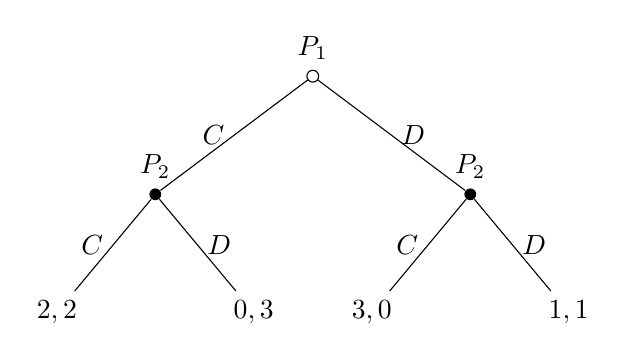
\begin{tikzpicture}[thin,
		level 1/.style={sibling distance=40mm},
		level 2/.style={sibling distance=25mm},
		level 3/.style={sibling distance=15mm},
		every circle node/.style={minimum size=1.5mm,inner sep=0mm}]
		
		\node[circle,draw,label=above:$P_{1}$] (root) {}
		child { node [circle,fill,label=above:$P_{2}$] {}
			child { 
				node {$2,2$}
				edge from parent
				node[left] {$C$}}
			child { 
				node {$0,3$} % [double] specifies the double line
				edge from parent
				node[right] {$D$}}
			edge from parent
			node[left] {$C$}}
		child { node [circle,fill,label=above:$P_{2}$] {}
			child { 
				node {$3,0$}
				edge from parent
				node[left] {$C$}}
			child { 
				node {$1,1$}
				edge from parent
				node[right] {$D$}}
			edge from parent
			node[right] {$D$}};
		\end{tikzpicture}
	\end{center}
\end{example}



\begin{theorem}[existence of pure strategy Nash equilibrium]
Every (finite) perfect-information game in extensive form has at least one pure-strategy Nash equilibrium.	
\end{theorem}

\subsection{Backward induction algorithm}

\section{Dynamic games with complete information}

\section{Multiobjective optimization}
\subsection{Basic concepts}
\begin{definition}\cite[18]{collette2013multiobjective}\index{multiobjective optimization}
A multiobjective optimization problem is defined as
\begin{align*}
    \min_{x\in \R^n} f(x) &= (f_1(x),f_2(x),...,f_k(x)),k\geq 2\\
    \text{subject to} ~ & g_i(x)\leq 0,i=1,2...,p \\
    & h_i(x)=0,i=1,2...,q
\end{align*}
\end{definition}

\begin{definition}[ideal objective vector]\cite[39]{collette2013multiobjective}\index{ideal point}
The ideal point of the objective function vector is a vector with each component minimized separately. The ideal point represents the best situation in optimizing the multiobjective function.
\end{definition}


\subsection{Pareto optimality}
\begin{definition}[domination relation]\index{domination}
In the multiojective optimization problem, a vector $x_1$ dominates $x_2$ if
\begin{itemize}
    \item $f_i(x_1) \leq f_i(x_2),\forall i$
    \item there exist one $i$ such that $f_i(x_1) < f_(x_2)$
\end{itemize}
\end{definition}

\begin{remark}
The domination relation express the intuitive meaning of 'better'.
\end{remark}

\begin{definition}[local optimality in the Pareto sense]\cite[19]{collette2013multiobjective}\index{local Pareto optimal}
A vector $x^*\in \R^n$ is locally optimal in the Pareto sense if there exists a real $\delta > 0$ such that for all $x \in \{x:\norm{x-x^*}\leq \delta\}$, $x$ does not dominate $x^*$.
\end{definition}


\begin{definition}[global optimality in the Pareto sense]\cite[19]{collette2013multiobjective}\index{global Pareto optimal}
A vector $x^*\in \R^n$ is locally optimal in the Pareto sense if there exists a real $\delta > 0$ such that for all $x \in \{x:\norm{x-x^*}\leq \delta\}$, $x$ does not dominate $x^*$.
\end{definition}


\section{Notes on bibliography}

A good resource on zero-sum game is at \href{http://math.ucr.edu/home/baez/games/}{link}.

\cite{gibbons1992game}\cite{fudenberg1991game}
For introduction to multiobjective optimization, see \cite{collette2013multiobjective}.
For good treatment on theory and method, see \cite{miettinen2012nonlinear}.
\printbibliography
\end{refsection}